\documentclass[12pt, twoside]{article}
\input{../preamble}
\usepackage{pgfplots}
\pgfplotsset{compat=1.18}

\fancyhead[LE]{\thepage}
\fancyhead[RO]{\thepage}
\fancyhead[LO]{La Scuola d'Italia / Dr.\ Huson / IB Math \\* 1 April 2026 --- Markscheme}

\begin{document}
\subsubsection*{6.5 Classwork: Quadratic Functions and Symmetry --- Markscheme}

\begin{enumerate}[itemsep=0.2cm]

%--- Problem 1: Graph to factored and standard form [7 marks] ---
\item The diagram shows the graph of a quadratic function with
$x$-intercepts at $(1, 0)$ and $(5, 0)$.

\begin{enumerate}[itemsep=0.15cm]
  \item Find the equation of the axis of symmetry. \hfill [1]
  \item Write the equation of the parabola in factored form, $y = (x - p)(x - q)$. \hfill [1]
  \item Expand to show that the equation is $y = x^2 - 6x + 5$. \hfill [2]
  \item Find the coordinates of the vertex. \hfill [2]
  \item Write down the $y$-intercept. \hfill [1]
\end{enumerate}

\vfill
\begin{tikzpicture}
  \draw (0,0) rectangle (15.5,10);
  \node[anchor=north west, inner sep=0.40cm] at (0,10) {%
    \begin{minipage}[t]{14.7cm}%
      \textbf{Solutions}\\[0.4cm]
      \textbf{(a)}\enspace $x = \dfrac{1 + 5}{2} = 3$ \hfill \textbf{(A1)}\\[0.4cm]
      The axis of symmetry is $x = 3$.\\[0.4cm]
      \textbf{(b)}\enspace $y = (x - 1)(x - 5)$ \hfill \textbf{(A1)}\\[0.4cm]
      \textbf{(c)}\enspace $y = (x - 1)(x - 5)$\\[0.2cm]
      \hspace*{2.5em}$= x^2 - 5x - x + 5$ \hfill \textbf{(M1)}\\[0.2cm]
      \hspace*{2.5em}$= x^2 - 6x + 5$ \hfill \textbf{(AG)}\\[0.4cm]
      \textbf{(d)}\enspace $y = (3)^2 - 6(3) + 5 = 9 - 18 + 5 = -4$ \hfill \textbf{(M1)}\\[0.2cm]
      \hspace*{2.5em}Vertex: $(3,\, -4)$ \hfill \textbf{(A1)}\\[0.4cm]
      \textbf{(e)}\enspace $y$-intercept: $x = 0$, $y = 0 - 0 + 5 = 5$, so $(0,\, 5)$ \hfill \textbf{(A1)}
    \end{minipage}%
  };
\end{tikzpicture}

\newpage

%--- Problem 2: Vertex form to standard form [7 marks] ---
\item The diagram shows the graph of $g(x) = -(x - 2)^2 + 9$.

\begin{enumerate}[itemsep=0.15cm]
  \item Write down the coordinates of the vertex. \hfill [1]
  \item Write down the equation of the axis of symmetry. \hfill [1]
  \item Show that $g(x) = -x^2 + 4x + 5$. \hfill [2]
  \item Solve $g(x) = 0$ to find the $x$-intercepts. \hfill [3]
\end{enumerate}

\vfill
\begin{tikzpicture}
  \draw (0,0) rectangle (15.5,12);
  \node[anchor=north west, inner sep=0.40cm] at (0,12) {%
    \begin{minipage}[t]{14.7cm}%
      \textbf{Solutions}\\[0.4cm]
      \textbf{(a)}\enspace Vertex: $(2,\, 9)$ \hfill \textbf{(A1)}\\[0.4cm]
      \textbf{(b)}\enspace $x = 2$ \hfill \textbf{(A1)}\\[0.4cm]
      \textbf{(c)}\enspace $g(x) = -(x - 2)^2 + 9$\\[0.2cm]
      \hspace*{2.5em}$= -(x^2 - 4x + 4) + 9$ \hfill \textbf{(M1)}\\[0.2cm]
      \hspace*{2.5em}$= -x^2 + 4x - 4 + 9$\\[0.2cm]
      \hspace*{2.5em}$= -x^2 + 4x + 5$ \hfill \textbf{(AG)}\\[0.4cm]
      \textbf{(d)}\enspace $-x^2 + 4x + 5 = 0$\\[0.2cm]
      \hspace*{2.5em}$x^2 - 4x - 5 = 0$ \quad (multiply both sides by $-1$) \hfill \textbf{(M1)}\\[0.2cm]
      \hspace*{2.5em}$(x - 5)(x + 1) = 0$ \hfill \textbf{(M1)}\\[0.2cm]
      \hspace*{2.5em}$x = 5$ or $x = -1$ \hfill \textbf{(A1)}\\[0.2cm]
      \hspace*{2.5em}The $x$-intercepts are $(-1,\, 0)$ and $(5,\, 0)$.
    \end{minipage}%
  };
\end{tikzpicture}

\newpage

%--- Problem 3: Standard form to factored and vertex form [7 marks] ---
\item The diagram shows the graph of $h(x) = x^2 - 2x - 3$.

\begin{enumerate}[itemsep=0.15cm]
  \item Write $h(x)$ in factored form, $(x - p)(x - q)$. \hfill [2]
  \item Write down the $x$-intercepts of the parabola. \hfill [1]
  \item Find the equation of the axis of symmetry. \hfill [1]
  \item Find the coordinates of the vertex. \hfill [2]
  \item Write $h(x)$ in vertex form, $(x - h)^2 + k$. \hfill [1]
\end{enumerate}

\vfill
\begin{tikzpicture}
  \draw (0,0) rectangle (15.5,11);
  \node[anchor=north west, inner sep=0.40cm] at (0,11) {%
    \begin{minipage}[t]{14.7cm}%
      \textbf{Solutions}\\[0.4cm]
      \textbf{(a)}\enspace Find two numbers that multiply to $-3$ and add to $-2$: \hfill \textbf{(M1)}\\[0.2cm]
      \hspace*{2.5em}$h(x) = (x + 1)(x - 3)$ \hfill \textbf{(A1)}\\[0.4cm]
      \textbf{(b)}\enspace $x$-intercepts: $(-1,\, 0)$ and $(3,\, 0)$ \hfill \textbf{(A1)}\\[0.4cm]
      \textbf{(c)}\enspace $x = \dfrac{-1 + 3}{2} = 1$ \hfill \textbf{(A1)}\\[0.4cm]
      \textbf{(d)}\enspace $h(1) = (1)^2 - 2(1) - 3 = 1 - 2 - 3 = -4$ \hfill \textbf{(M1)}\\[0.2cm]
      \hspace*{2.5em}Vertex: $(1,\, -4)$ \hfill \textbf{(A1)}\\[0.4cm]
      \textbf{(e)}\enspace $(x - 1)^2 - 4$ \hfill \textbf{(A1)}
    \end{minipage}%
  };
\end{tikzpicture}

\newpage

%--- Problem 4: Sketch from factored form [8 marks] ---
\item Consider the quadratic function $p(x) = -x(x - 4)$ with domain $-1 \leq x \leq 5$.

\begin{enumerate}[itemsep=0.15cm]
  \item Write down the $x$-intercepts. \hfill [1]
  \item Find the equation of the axis of symmetry. \hfill [1]
  \item Find the coordinates of the vertex. \hfill [2]
  \item Expand to write $p(x)$ in the form $ax^2 + bx + c$. \hfill [1]
  \item On the grid below, sketch the graph of $p(x)$. Label the vertex
        and $x$-intercepts. \hfill [2]
  \item Write down the range of the function over the given domain. \hfill [1]
\end{enumerate}

\vfill
\begin{tikzpicture}
  \draw (0,0) rectangle (15.5,5);
  \node[anchor=north west, inner sep=0.40cm] at (0,5) {%
    \begin{minipage}[t]{14.7cm}%
      \textbf{Solutions}\\[0.4cm]
      \textbf{(a)}\enspace $x$-intercepts: $(0,\, 0)$ and $(4,\, 0)$ \hfill \textbf{(A1)}\\[0.4cm]
      \textbf{(b)}\enspace $x = \dfrac{0 + 4}{2} = 2$ \hfill \textbf{(A1)}\\[0.4cm]
      \textbf{(c)}\enspace $p(2) = -2(2 - 4) = -2(-2) = 4$. \quad Vertex: $(2,\, 4)$ \hfill \textbf{(M1)(A1)}\\[0.4cm]
      \textbf{(d)}\enspace $p(x) = -x^2 + 4x$ \hfill \textbf{(A1)}
    \end{minipage}%
  };
\end{tikzpicture}

\vspace{0.3cm}
\textbf{(e)} Graph: downward-opening parabola through $(0,\, 0)$ and $(4,\, 0)$
with vertex at $(2,\, 4)$. \hfill \textbf{(A1)} shape, \textbf{(A1)} key points

\begin{center}
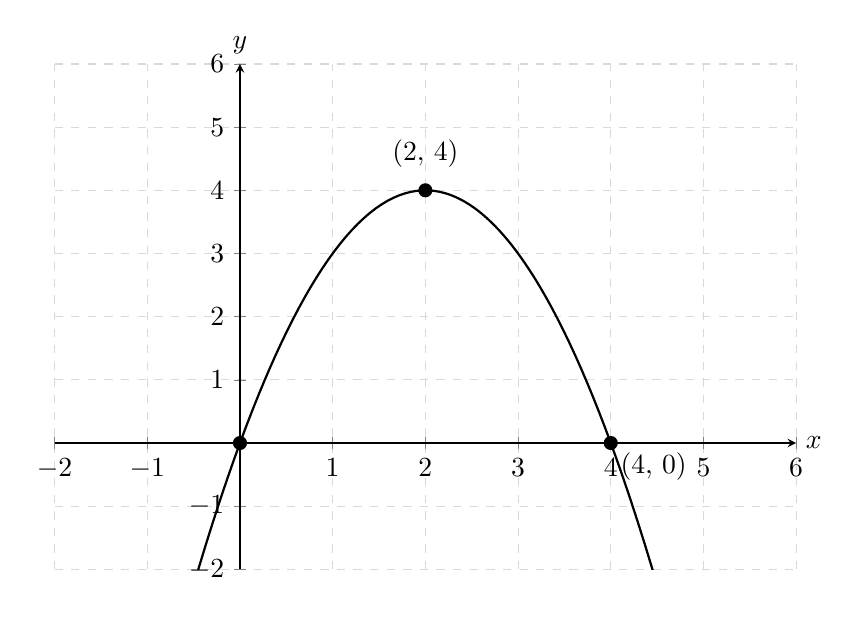
\begin{tikzpicture}
\begin{axis}[
  axis lines=middle,
  xlabel={$x$},
  ylabel={$y$},
  grid=both,
  grid style={dashed, gray!30},
  xmin=-2, xmax=6,
  ymin=-2, ymax=6,
  xtick={-2,-1,...,6},
  ytick={-2,-1,...,6},
  width=11cm,
  height=8cm,
  every axis x label/.style={at={(ticklabel* cs:1.0)}, anchor=west},
  every axis y label/.style={at={(ticklabel* cs:1.0)}, anchor=south},
]
  % Solution curve
  \addplot[thick, domain=-0.5:4.5, samples=80] {-x^2 + 4*x};
  % Key points
  \node[circle, fill, inner sep=1.8pt] at (axis cs:0,0) {};
  \node[circle, fill, inner sep=1.8pt] at (axis cs:4,0) {};
  \node[circle, fill, inner sep=1.8pt] at (axis cs:2,4) {};
  % Labels
  \node[anchor=south] at (axis cs:2,4.2) {$(2,\, 4)$};
  \node[anchor=north west] at (axis cs:4,0) {$(4,\, 0)$};
\end{axis}
\end{tikzpicture}
\end{center}

\vspace{0.3cm}
\textbf{(f)} Over the domain $-1 \leq x \leq 5$, the vertex gives the maximum
$p(2) = 4$, and the endpoints give the minimum: $p(-1) = -(-1)(-5) = -5$ and
$p(5) = -(5)(1) = -5$. \hfill \textbf{(A1)}\\[0.2cm]
\hspace*{1.5em}Range: $-5 \leq p(x) \leq 4$.

\end{enumerate}
\end{document}
